\chapter{User Interface and User Experience (Patient and Doctor Apps)}
\label{ch:ui-ux}

\section{Overview}

This chapter documents the user interface (UI) and user experience (UX) of the patient and doctor applications. The screenshots are grouped by application and by primary workflow intent (onboarding, scheduling, documentation, and video consultation).

To keep the layout consistent and readable, screenshots are displayed in a two-up grid (two images per figure row). Each figure row contains a shared caption describing the two screens shown.

\section{Wireframing to UI Solution}

The interface concepts were developed through iterative wireframing before producing the final high-fidelity UI screens. To illustrate this process transparently, the following figures include the complete patient-app wireframe set. The doctor-app UI was developed through the same workflow-first wireframing approach; representative final screens are shown in the next section.

\newcommand{\TwoUpWireP}[4]{%
  \begin{figure}[H]
  \centering
  \setlength{\fboxsep}{0pt}
  \begin{minipage}{0.48\linewidth}
    \centering
    \fbox{\includegraphics[width=\linewidth,height=0.26\textheight,keepaspectratio]{#1}}
  \end{minipage}\hfill
  \begin{minipage}{0.48\linewidth}
    \centering
    \fbox{\includegraphics[width=\linewidth,height=0.26\textheight,keepaspectratio]{#2}}
  \end{minipage}
  \caption{Patient wireframes: #3}
  \label{#4}
  \end{figure}
}

\TwoUpWireP{ux_wireframes/patient/wireframe_get_started_p.png}{ux_wireframes/patient/wireframe_sign_in_p.png}{Get started and sign-in entry}{fig:wf_patient_entry}
\TwoUpWireP{ux_wireframes/patient/wireframe_create_account_p.png}{ux_wireframes/patient/wireframe_create_p.png}{Create account and registration (step 1)}{fig:wf_patient_create_1}
\TwoUpWireP{ux_wireframes/patient/wireframe_create_p_1.png}{ux_wireframes/patient/wireframe_create_p_2.png}{Registration flow (steps 2--3)}{fig:wf_patient_create_2}
\TwoUpWireP{ux_wireframes/patient/wireframe_create_p_3.png}{ux_wireframes/patient/wireframe_account_success_p.png}{Registration (final step) and success}{fig:wf_patient_create_3}
\TwoUpWireP{ux_wireframes/patient/wireframe_home_p.png}{ux_wireframes/patient/wireframe_bookings_p.png}{Home and bookings overview}{fig:wf_patient_home_bookings}
\TwoUpWireP{ux_wireframes/patient/wireframe_appointment_details_p.png}{ux_wireframes/patient/wireframe_documents_p.png}{Appointment details and documents list}{fig:wf_patient_appt_docs}
\TwoUpWireP{ux_wireframes/patient/wireframe_documents_p_1.png}{ux_wireframes/patient/wireframe_profile_p.png}{Document detail and profile}{fig:wf_patient_docs_profile}
\TwoUpWireP{ux_wireframes/patient/wireframe_profile_image_p.png}{ux_wireframes/patient/wireframe_account_info_p.png}{Profile image and account information}{fig:wf_patient_profile_account}

\section{Doctor App UI Screens}

The following sections present the realized UI screens of both applications. While the wireframes capture structure and workflow intent, the final screens refine visual hierarchy, typography, and interaction affordances for practical daily use.

\newcommand{\TwoUpDoctor}[5]{%
  \begin{figure}[H]
  \centering
  \setlength{\fboxsep}{0pt}
  \begin{minipage}{0.48\linewidth}
    \centering
    \fbox{\includegraphics[width=\linewidth,height=0.26\textheight,keepaspectratio]{#1}}
  \end{minipage}\hfill
  \begin{minipage}{0.48\linewidth}
    \centering
    \fbox{\includegraphics[width=\linewidth,height=0.26\textheight,keepaspectratio]{#2}}
  \end{minipage}
  \caption{Doctor app screens: #5}
  \end{figure}
}

\TwoUpDoctor{ui_screens/doctor/doctor_loading_1.jpg}{ui_screens/doctor/doctor_loading_2.jpg}{Loading screen (variant 1)}{Loading screen (variant 2)}{Loading and initialization}
\TwoUpDoctor{ui_screens/doctor/doctor_create_account.jpg}{ui_screens/doctor/doctor_create_account_confirm.jpg}{Create account}{Account creation confirmation}{Doctor onboarding}
\TwoUpDoctor{ui_screens/doctor/doctor_account_information.jpg}{ui_screens/doctor/doctor_profile_image.jpg}{Account information}{Profile image}{Account setup}
\TwoUpDoctor{ui_screens/doctor/doctor_profile.jpg}{ui_screens/doctor/doctor_home.jpg}{Doctor profile}{Doctor home dashboard}{Profile and daily work}

\TwoUpDoctor{ui_screens/doctor/doctor_calendar_setup_intro.jpg}{ui_screens/doctor/doctor_calendar_setup_1.jpg}{Calendar setup introduction}{Availability input}{Calendar setup}
\TwoUpDoctor{ui_screens/doctor/doctor_calendar_setup_2.jpg}{ui_screens/doctor/doctor_calendar_setup_3.jpg}{Slot configuration}{Exceptions/controls}{Scheduling rules}
\TwoUpDoctor{ui_screens/doctor/doctor_calendar_setup_4.jpg}{ui_screens/doctor/doctor_calendar_setup_5.jpg}{Review and persistence}{Final confirmation}{Calendar finalization}

\TwoUpDoctor{ui_screens/doctor/doctor_patients.jpg}{ui_screens/doctor/doctor_attach_patient.jpg}{Patients list}{Attach patient context}{Patient context workflow}
\TwoUpDoctor{ui_screens/doctor/doctor_schedule_edit.jpg}{ui_screens/doctor/doctor_documents.jpg}{Schedule edit}{Document management}{Availability updates and records}

\TwoUpDoctor{ui_screens/doctor/doctor_start_appointment.jpg}{ui_screens/doctor/doctor_start_appointment_confirm.jpg}{Start appointment}{Start appointment confirmation}{Encounter initiation}

% Odd number of screenshots: the remaining screen is shown as a single figure.
\begin{figure}[H]
\centering
\setlength{\fboxsep}{0pt}
\fbox{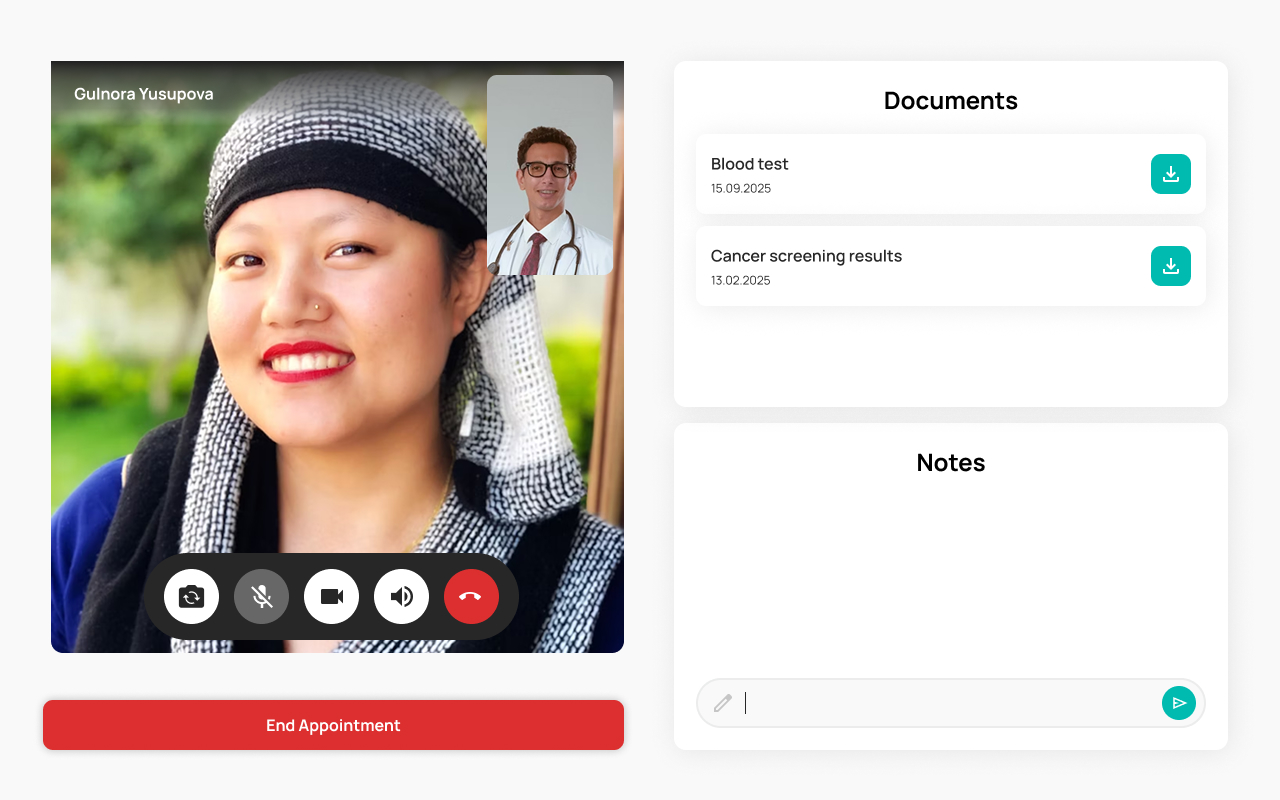
\includegraphics[width=0.72\linewidth,height=0.26\textheight,keepaspectratio]{ui_screens/doctor/doctor_join_video.jpg}}
\caption{Doctor app: video consultation join}
\end{figure}

\section{Patient App UI Screens}

\newcommand{\TwoUpPatient}[5]{%
  \begin{figure}[H]
  \centering
  \setlength{\fboxsep}{0pt}
  \begin{minipage}{0.48\linewidth}
    \centering
    \fbox{\includegraphics[width=\linewidth,height=0.26\textheight,keepaspectratio]{#1}}
  \end{minipage}\hfill
  \begin{minipage}{0.48\linewidth}
    \centering
    \fbox{\includegraphics[width=\linewidth,height=0.26\textheight,keepaspectratio]{#2}}
  \end{minipage}
  \caption{Patient app screens: #5}
  \end{figure}
}

\TwoUpPatient{ui_screens/patient/patient_loading.png}{ui_screens/patient/patient_loading_2.png}{Loading screen (variant 1)}{Loading screen (variant 2)}{Startup and readiness}
\TwoUpPatient{ui_screens/patient/patient_get_started.png}{ui_screens/patient/patient_create_account.png}{Get started}{Create account}{Onboarding}

\TwoUpPatient{ui_screens/patient/patient_create_flow_1.png}{ui_screens/patient/patient_create_flow_2.png}{Create flow step 1}{Create flow step 2}{Account creation flow}
\TwoUpPatient{ui_screens/patient/patient_create_flow_3.png}{ui_screens/patient/patient_create_flow_4.png}{Create flow step 3}{Create flow step 4}{Account creation flow (continued)}
\TwoUpPatient{ui_screens/patient/patient_create_flow_5.png}{ui_screens/patient/patient_home.png}{Create flow step 5}{Home}{Account confirmation and home}

\TwoUpPatient{ui_screens/patient/patient_bookings.png}{ui_screens/patient/patient_doctors.png}{Bookings}{Doctors list}{Selecting a provider}
\TwoUpPatient{ui_screens/patient/patient_doctors_detail.png}{ui_screens/patient/patient_documents.png}{Doctor details}{Documents list}{Provider overview and records}
\TwoUpPatient{ui_screens/patient/patient_documents_detail.png}{ui_screens/patient/patient_profile.png}{Document detail}{Profile overview}{Viewing documents and profile}

\TwoUpPatient{ui_screens/patient/patient_profile_menu.png}{ui_screens/patient/patient_profile_image.png}{Profile menu}{Profile image}{Profile settings}
\TwoUpPatient{ui_screens/patient/patient_account_info.png}{ui_screens/patient/patient_appointment_upcoming.png}{Account info}{Upcoming appointment}{Appointments overview}
\TwoUpPatient{ui_screens/patient/patient_appointment_upcoming_2.png}{ui_screens/patient/patient_appointment_past.png}{Upcoming details (variant)}{Past appointment}{Appointment details}
\TwoUpPatient{ui_screens/patient/patient_waiting_room.png}{ui_screens/patient/patient_video_call.png}{Waiting room}{Video consultation}{Video encounter}

\section{Cross-Cutting UX Considerations}

Across both applications, the UX is organized around clinical intent units: (1) confirm identity and session integrity, (2) establish appointment context, (3) communicate and exchange supporting information, and (4) preserve continuity of care through documents and encounter summaries.

The doctor application emphasizes availability configuration and encounter initiation as primary first-class actions. The patient application emphasizes booking discoverability and appointment awareness through lists and detail screens. Both clients support asynchronous workflow continuity via tasks and notifications.

The present chapter therefore focuses on design and implemented interaction structure, while the evaluation design and methodological framing for assessing usability, acceptability, and perceived impact are discussed in later chapters as part of the ongoing prototype evaluation.

